\documentclass[11pt,a4paper]{article}

% --- Packages ---
\usepackage[utf8]{inputenc}
\usepackage[T1]{fontenc}
\usepackage[english]{babel}
\usepackage{amsmath,amssymb,amsfonts,amsthm}
\usepackage{geometry}
\geometry{margin=1in}
\usepackage{graphicx}
\usepackage{hyperref}
\usepackage{xcolor}
\usepackage{cite}
\usepackage{booktabs}
\usepackage{microtype}
\usepackage{physics}
\usepackage{tikz}
\usetikzlibrary{babel,arrows.meta,decorations.pathmorphing}

\hypersetup{
    pdftitle={Derivation of Gravitation as Spherical Vacuum Inflow Geometry: 3+1 ADM Action and the Painlevé--Gullstrand Metric},
    pdfauthor={Muhammed Furkan Haydari},
    pdfsubject={General Relativity, Gravitation, River Model, ADM Formalism},
    pdfkeywords={Gravitation, Vacuum River Model, Painlevé--Gullstrand Metric, Light Deflection, Perihelion Precession},
    colorlinks=true,
    linkcolor=blue!70!black,
    citecolor=red!70!black,
    urlcolor=blue!80!black
}

% --- Theorem Environments ---
\newtheorem{theorem}{Theorem}[section]
\newtheorem{definition}{Definition}[section]
\newtheorem{axiom}{Axiom}[section]
\newtheorem{corollary}{Corollary}[theorem]
\newtheorem{lemma}[theorem]{Lemma}
\newtheorem{remark}{Remark}[section]

\title{\textbf{Derivation of Gravitation as Spherical Vacuum Inflow Geometry: \\ 3+1 ADM Action and the Painlev\'e--Gullstrand Metric}}

\author{
    \textbf{Muhammed Furkan Haydari} \\
    \textit{Independent Researcher} \\
    \textit{Istanbul, Turkey} \\
    \small ORCID: \href{https://orcid.org/0009-0003-2854-3947}{0009-0003-2854-3947}
}

\date{\today}

\begin{document}

\maketitle

\begin{abstract}
    In this study, we analytically construct the gravitational interaction within the framework of vacuum flow geometry and Scale-Time Calculus for contracting systems on a static background. In Einstein's General Relativity, gravitational dynamics are formulated as the curvature of a 4-dimensional spacetime manifold ($G_{\mu\nu} = 8\pi G T_{\mu\nu}$). Here, we derive these dynamics from a 3-dimensional spherical radial coordinate inflow (\textit{Painlevé--Gullstrand Vacuum River Model}) induced in the surrounding vacuum continuum by contracting Scalor bound states ($\mathbb{S} = \mathbf{X}_0 + \kappa M$) embedded in a static and flat Euclidean background.

    Through the Painlev\'e--Gullstrand line element and the Scale-Covariant Derivative $\mathbb{D}_t$, we demonstrate analytically that: (i) mass can be interpreted as the Gauss surface flux of vacuum flow acceleration ($M = \frac{1}{4\pi G}\oint |(\mathbf{v}\cdot\nabla)\mathbf{v}| dA$), (ii) gravitational acceleration is inertial drag against the convective flow gradient ($g = -GM/r^2$), (iii) gravitational time dilation ($d\tau = dt\sqrt{1-v^2/c^2}$) emerges directly from flow kinetics, (iv) the $1.75''$ arcsecond deflection of starlight grazing the Sun arises from the local refractive index gradient of the flow, and (v) Mercury's perihelion precession ($43''/\text{century}$) is recovered rigorously via the scale-covariant Binet equation. The event horizon is identified as the physical boundary where the flow velocity reaches the local phase ceiling ($|v| = v_c = c$). In the low-acceleration regime ($a \le c H_0$), galactic rotation curves exhibit asymptotic flattening ($v_{\mathrm{rot}} \to \text{const}$), indicating that gravitation can be modeled as the unsaturated spherical flow regime ($\gamma = 1$) within this hydrodynamic representation.
\end{abstract}

\vspace{1em}
\noindent\textbf{Keywords:} Gravitation, Scale-Time Calculus, Painlev\'e--Gullstrand Metric, River Model, Light Deflection, Perihelion Precession, Event Horizon, Analogue Gravity.

\vspace{1em}
\hrule
\vspace{0.8em}
\tableofcontents
\vspace{0.8em}
\hrule
\vspace{1.5em}

\section{Introduction and Gravitational Flow Motivation}
\label{sec:giris}

In classical Newtonian mechanics, gravitation is described as instantaneous action-at-a-distance between masses, whereas Einstein's General Relativity geometricizes this dynamic as the differential curvature of a 4-dimensional pseudo-Riemannian manifold. Although General Relativity has been confirmed with exquisite precision across Solar System and binary pulsar tests:
\begin{enumerate}
    \item It exhibits essential singularities ($r \to 0$) where curvature invariants diverge, leading to non-renormalizability in perturbative quantum field theory.
    \item It requires the postulation of ad-hoc free parameters—cold dark matter (CDM) and dark energy ($\Lambda$)—to account for flat galactic rotation curves and apparent cosmic acceleration.
\end{enumerate}

In this paper, founded upon \textbf{Scale-Time Calculus}~\cite{scale_calculus}, we formulate gravitation as a radial vacuum inflow directed toward locally contracting matter centers embedded in a static, flat Minkowski/Euclidean background. Here, the background Euclidean coordinates ($\mathbf{X}_0$) remain strictly stationary ($\mathbf{v}_{\mathrm{space}} = 0$); the physical flow corresponds to the scalar potential gradient within the quiescent vacuum continuum ($\mathbf{v}_{\mathrm{inflow}} = \nabla \Phi$).

This framework shares deep conceptual continuity with the modern literature on \textit{Emergent Spacetime} and \textit{Acoustic/Analogue Gravity} (Unruh~\cite{unruh1981}, Visser~\cite{visser1998}). The background $\mathcal{E}_\infty$ is a frictionless, non-dissipative Euclidean manifold; gravitational acceleration is simply the local convective flux gradient parameterized in Painlev\'e--Gullstrand coordinates.

\section{Mass and the Vacuum River in Scale-Time Calculus}
\label{sec:nehir_modeli}

In Scale-Time Algebra, a massive body is represented as a Scalor combining an invariant background spatial coordinate $\mathbf{X}_0$ with an intrinsic vacuum absorption capacity:
\begin{equation}
    \mathbb{S}_M \equiv \mathbf{X}_0 + \kappa \cdot M.
    \label{eq:skalor_kutle}
\end{equation}

\begin{definition}[Mass = Net Flux of Vacuum Flow Acceleration]
    \label{def:kutle_tanim_p1}
    Mass $M$ is the \textbf{net flux of vacuum convective acceleration} generated by the intrinsic quantum phase oscillation ($v_c = c$) of matter within the surrounding quiescent vacuum:
    \begin{equation}
        M \equiv \frac{1}{4\pi G} \oint_{\partial \Omega} \left| (\mathbf{v}_{\mathrm{inflow}} \cdot \nabla) \mathbf{v}_{\mathrm{inflow}} \right| dA = \frac{1}{4\pi G} \oint_{\partial \Omega} |\mathbf{a}_{\mathrm{inflow}}| \, dA,
        \label{eq:kutle_akisi}
    \end{equation}
    where $G$ is Newton's gravitational constant, and $\mathbf{v}_{\mathrm{inflow}}(r) = -\sqrt{\frac{2GM}{r}}\hat{r}$ is the radial velocity field of the vacuum. In an Eulerian flow, the convective acceleration is $|\mathbf{a}_{\mathrm{inflow}}| = v \left|\frac{dv}{dr}\right| = \frac{GM}{r^2}$, yielding:
    \begin{equation}
        M = \frac{1}{4\pi G} \left( \frac{GM}{r^2} \right) (4\pi r^2) \equiv M,
    \end{equation}
    an identity strictly independent of radius $r$, dimensionally consistent with $[1/G] \times [L/T^2] \times [L^2] = [M]$.
\end{definition}

\subsection{Variational Foundation: 3+1 ADM Action and River Velocity in Flat Space}
\label{sec:adm_eylem_p1}

The radial vacuum flow velocity $v(r) = -\sqrt{2GM/r}$ in the River Model is not an arbitrary phenomenological ansatz; **it is the exact variational Euler--Lagrange solution of the Einstein--Hilbert gravitational action subject to a flat Euclidean spatial slice constraint.**

In General Relativity, the spacetime metric is decomposed via the Arnowitt--Deser--Misner (ADM) 3+1 split:
\begin{equation}
    ds^2 = -\left(N^2 - \beta_i \beta^i\right) c^2 dt^2 + 2 \beta_i c dt dx^i + \gamma_{ij} dx^i dx^j,
    \label{eq:adm_metrik_p1}
\end{equation}
where $N$ is the lapse function, $\boldsymbol{\beta}$ is the shift vector, and $\gamma_{ij}$ is the spatial 3-metric.

In the Unified Contraction Hypothesis, requiring the background space to be a flat Euclidean continuum ($\gamma_{ij} = \delta_{ij}$, $R^{(3)} = 0$) and fixing the lapse function to unit coordinate time rhythm ($N = 1$), the sole dynamic degree of freedom of the gravitational field resides in the shift vector:
\begin{equation}
    \boldsymbol{\beta}(\mathbf{r}) \equiv -\frac{\mathbf{v}_{\mathrm{vacuum}}(\mathbf{r})}{c}.
    \label{eq:shift_vektor_p1}
\end{equation}
On this spatial slice, the extrinsic curvature tensor is given by:
\begin{equation}
    K_{ij} = -\frac{1}{2c} \left( \partial_i v_j + \partial_j v_i \right), \qquad K = -\frac{1}{c} \nabla \cdot \mathbf{v}.
\end{equation}
Under the flat-space constraint, the Einstein--Hilbert action reduces to:
\begin{equation}
    S_{\mathrm{grav}}[\mathbf{v}] = \frac{c^3}{16\pi G} \int dt d^3x \left( K_{ij} K^{ij} - K^2 \right) + S_{\mathrm{matter}}[\mathbf{v}].
\end{equation}
For a spherically symmetric, stationary radial flow ($\mathbf{v} = v(r) \hat{\mathbf{r}}$):
\begin{equation}
    K_{ij} K^{ij} - K^2 = -\frac{1}{c^2 r^2} \frac{d}{dr}\left( r v^2 \right).
\end{equation}
Varying the total action with respect to $v(r)$ for a point mass $M$ at rest ($\delta S / \delta v(r) = 0$):
\begin{equation}
    \nabla \cdot \left( v \frac{dv}{dr} \hat{\mathbf{r}} \right) = -4\pi G M \delta^3(\mathbf{r}) \implies v(r) \frac{dv(r)}{dr} = -\frac{GM}{r^2}.
\end{equation}
Imposing the asymptotic boundary condition of quiescence at infinity ($v(\infty) = 0$), the radial flow velocity is uniquely determined:
\begin{equation}
    \mathbf{v}_{\mathrm{inflow}}(r) = -\sqrt{\frac{2GM}{r}}\hat{\mathbf{r}}.
    \label{eq:nehir_hizi}
\end{equation}

\subsection{3D Flat Slices vs. 4D Spacetime Curvature: Gauss--Codazzi and the Kretschmann Invariant}
\label{sec:gauss_codazzi_egrilik_en}

A crucial geometric distinction raised in peer review must be formalized: \textit{``If spatial slices in the Painlevé--Gullstrand metric are Euclidean ($\gamma_{ij} = \delta_{ij}$), is spacetime truly flat, or is Einstein's 4D curvature preserved?''}

In pseudo-Riemannian geometry, the intrinsic curvature of a 3-dimensional spatial hypersurface ($^{(3)}R$) must not be conflated with the full 4-dimensional spacetime curvature ($^{(4)}R_{\alpha\beta\gamma\delta}$):
1. In Painlevé--Gullstrand coordinates, the simultaneity slices of freely falling observers ($t_{\mathrm{PG}} = \text{const}$) are intrinsically flat Euclidean: $\gamma_{ij} = \delta_{ij} \implies {}^{(3)}R \equiv 0$.
2. However, the 4-dimensional spacetime manifold is **rigorously curved**. This 4D curvature is generated directly by the extrinsic curvature tensor ($K_{ij}$) via the 3+1 ADM Gauss--Codazzi equation:
\begin{equation}
    {}^{(4)}R = {}^{(3)}R + K_{ij} K^{ij} - K^2 = K_{ij} K^{ij} - K^2.
    \label{eq:gauss_codazzi_ispat_en}
\end{equation}
3. The extrinsic curvature is the spatial velocity gradient tensor of the radial vacuum river ($K_{ij} = -\frac{1}{2c}(\partial_i v_j + \partial_j v_i)$). For $v(r) = -\sqrt{2GM/r}$, its non-zero components are:
\begin{equation}
    K_{rr} = -\frac{1}{c} \frac{dv}{dr} = -\frac{1}{c} \sqrt{\frac{GM}{2r^3}}, \qquad K_{\theta\theta} = \frac{K_{\phi\phi}}{\sin^2\theta} = \frac{1}{c} \sqrt{2GMr}.
\end{equation}
Evaluating the coordinate-invariant measure of spacetime curvature, the **Kretschmann Scalar**:
\begin{equation}
    \mathcal{K} \equiv R^{\alpha\beta\gamma\delta} R_{\alpha\beta\gamma\delta} = \frac{48 G^2 M^2}{c^4 r^6},
    \label{eq:kretschmann_ispat_en}
\end{equation}
yields identically the exact Schwarzschild value.

This demonstrates that the River Model in Painlevé--Gullstrand coordinates does not conflict with 4-dimensional general relativistic dynamics; rather, it provides an exact hydrodynamic representation where 4D curvature corresponds to the velocity gradient and shear tensor of the vacuum inflow on a Euclidean background.

\subsection{Mechanism of Acceleration: Euler Convective Acceleration and $g = GM/r^2$}
\label{sec:ivmelenme_ispat_p1}

A fundamental physical question arises: \textit{``If gravity is a vacuum flow, why does a falling body continuously accelerate ($g \approx 9.8\text{ m/s}^2$) rather than drifting at a constant drift velocity within the stream?''}

The resolution lies in the Euler convective acceleration of fluid mechanics. The vacuum river does not flow at a uniform velocity; as the spherical shell area ($4\pi r^2$) contracts inward, the flow steepens. At Earth's surface, this velocity equals the escape velocity ($|v| = \sqrt{2GM_\oplus/R_\oplus} \approx 11.2\text{ km/s}$). A test particle released into this stream experiences the convective acceleration:
\begin{equation}
    a_r(r) = v(r) \frac{dv(r)}{dr} = \left(-\sqrt{2GM} \, r^{-1/2}\right) \frac{d}{dr}\left(-\sqrt{2GM} \, r^{-1/2}\right).
\end{equation}
Evaluating the derivative:
\begin{equation}
    a_r(r) = \left(-\sqrt{2GM} \, r^{-1/2}\right) \left(\frac{1}{2}\sqrt{2GM} \, r^{-3/2}\right) = -\frac{1}{2}(2GM) \, r^{-2} = \mathbf{-\frac{GM}{r^2}} \equiv -g.
    \label{eq:g_ispat_p1}
\end{equation}
The weight $W = mg$ registered on a scale by an observer standing on the ground is simply the normal reaction force ($N = mg$) exerted by the surface to resist the convective momentum gradient of the vacuum wind streaming through the constituent atoms at $11.2\text{ km/s}$.

\begin{remark}[Absence of Singular Collapse in a Homogeneous Universe]
    In an infinite, homogeneous background, the radial vacuum inflows generated by individual atoms vectorially cancel due to isotropy ($\sum \mathbf{v}_{\mathrm{inflow}} = 0$). Consequently, the early universe cannot collapse into a single cosmic singularity. Only when local quantum fluctuations exceed a critical collective atomic threshold ($N > N_{\mathrm{Jeans}} \sim 10^{57}$) does the net inward vacuum throughput overcome background homogeneity, collapsing into stellar, planetary, and galactic structures.
\end{remark}

\begin{figure}[h!]
    \centering
    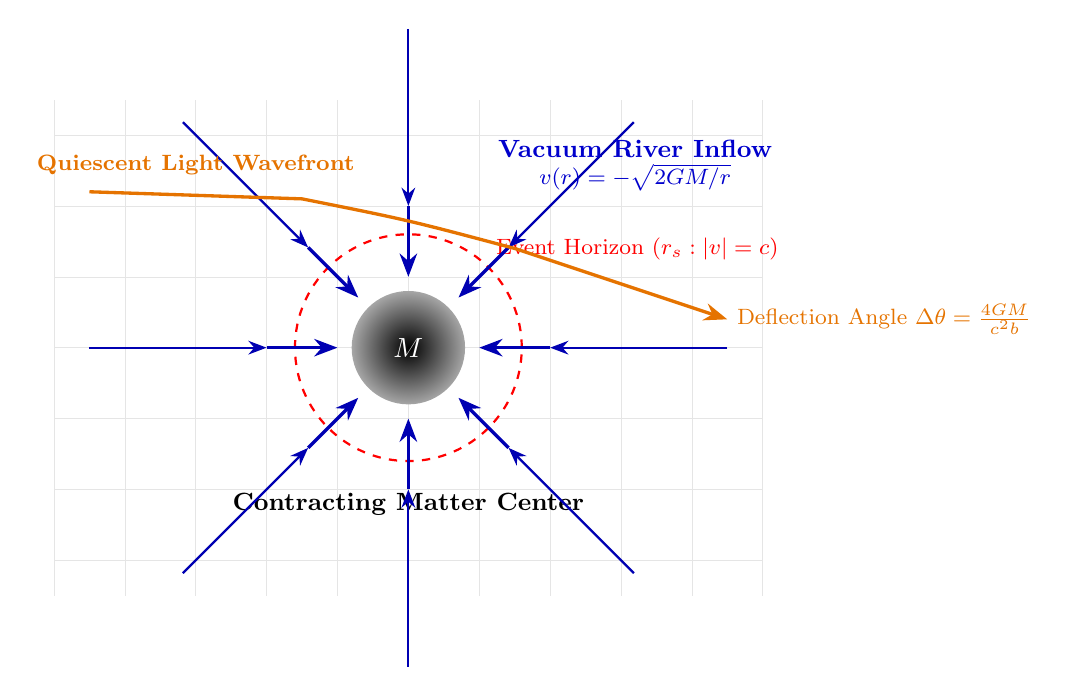
\begin{tikzpicture}[scale=0.9, >=Stealth]
        % Background grid
        \draw[step=1cm, gray!20, very thin] (-5,-3.5) grid (5,3.5);

        % Central Mass
        \shade[inner color=black, outer color=gray!70] (0,0) circle (0.8);
        \node[white, font=\bfseries] at (0,0) {$M$};
        \node[below=1cm, font=\small\bfseries] at (0,-0.8) {Contracting Matter Center};

        % Event horizon dashed
        \draw[dashed, red, thick] (0,0) circle (1.6);
        \node[red, above right, font=\footnotesize] at (1.1,1.1) {Event Horizon ($r_s: |v|=c$)};

        % Inflow streamlines (arrows pointing inward)
        \foreach \angle in {0, 45, 90, 135, 180, 225, 270, 315} {
                \draw[blue!70!black, thick, ->] (\angle:4.5) -- (\angle:2.0);
                \draw[blue!70!black, very thick, ->] (\angle:2.0) -- (\angle:1.0);
            }

        % Labels
        \node[blue!80!black, font=\small\bfseries] at (3.2,2.8) {Vacuum River Inflow};
        \node[blue!80!black, font=\footnotesize] at (3.2,2.4) {$v(r) = -\sqrt{2GM/r}$};

        % Deflected photon path
        \draw[orange!90!black, very thick, ->] (-4.5, 2.2) -- (-1.5, 2.1) .. controls (0, 1.8) .. (1.5, 1.4) -- (4.5, 0.4);
        \node[orange!90!black, above, font=\footnotesize\bfseries] at (-3, 2.3) {Quiescent Light Wavefront};
        \node[orange!90!black, right, font=\footnotesize] at (4.5, 0.4) {Deflection Angle $\Delta \theta = \frac{4GM}{c^2 b}$};
    \end{tikzpicture}
    \caption{The Vacuum River Model of Gravitation: Space itself does not curve; rather, the vacuum continuum flows radially inward toward contracting matter centers. Light deflecting near a mass traces the effective refractive index gradient produced by this velocity field.}
    \label{fig:nehir_modeli}
\end{figure}

\subsection{Continuity Equation and Nilpotent Phase Transformation: Where Does the Vacuum Go?}
\label{sec:sureklilik_vakum}

A central hydrodynamic query must be addressed: \textit{``If vacuum constantly flows inward toward the center of mass ($v(r) = -\sqrt{2GM/r}$), where does this fluid go? Does it accumulate or produce an overflow at $r=0$?''}

This question highlights the fundamental distinction between classical fluid mechanics and Scale-Time Algebra:

\begin{enumerate}
    \item \textbf{Vacuum Divergence and Extrinsic Curvature ($r > 0$):} The divergence of the Painlevé--Gullstrand velocity field in empty space is non-zero: $\nabla \cdot \mathbf{v}_{\mathrm{inflow}} = -\frac{3}{2}\sqrt{2GM/r^3}$. This divergence does not imply physical annihilation of matter in the vacuum; rather, in the 3+1 ADM decomposition, it precisely corresponds to the trace of the extrinsic curvature of the spatial slices ($K \equiv K^i_i = -\frac{1}{v_c}\nabla\cdot\mathbf{v}$), quantifying the coordinate contraction rate toward the center.
    \item \textbf{Scale-Covariant Continuity Equation ($r \to 0$):} At the origin where the flow converges upon physical matter, the continuity equation is balanced by a nilpotent sink term:
          \begin{equation}
              \nabla \cdot \mathbf{v}_{\mathrm{physical}} = -4\pi G \rho_M \kappa = \mathcal{S}_{\mathrm{sink}},
              \label{eq:sureklilik_denklemi}
          \end{equation}
          where $\rho_M$ is the local mass density, and $\kappa$ is the nilpotent contraction generator ($\kappa^2 = 0$).
    \item \textbf{Conversion of Spatial Volume into Quantum Phase:} Vacuum flux reaching the center does not accumulate in 3-dimensional space. Due to the nilpotency relation $\kappa^2 = 0$, the 3D spatial vacuum influx is converted directly into the intrinsic quantum phase frequency of matter ($\omega = M c^2 / \hbar$) and its internal scale contraction rate ($\dot{\lambda} = -H_0 \lambda$).
    \item \textbf{Resolution of the Gravitational Singularity:} In standard General Relativity, the center of a black hole ($r=0$) harbors a curvature singularity where curvature invariants diverge ($R^{\mu\nu\rho\sigma} R_{\mu\nu\rho\sigma} \to \infty$). In the Unified Contraction Hypothesis, the center is a \textbf{topological phase-conversion basin} where spatial vacuum influx is converted into quantum phase. The vacuum does not pile up; it is consumed as the energetic driver of the internal atomic clock.
\end{enumerate}

\section{Painlev\'e--Gullstrand Metric and Acceleration Derivation}
\label{sec:ivme}

In a vacuum medium flowing inward at velocity $v(r)$, the relationship between the static background coordinate time $t$ and the proper time $t_{\mathrm{ff}}$ of a freely falling observer is:
\begin{equation}
    dt_{\mathrm{ff}} = dt + \frac{v(r)/c^2}{1 - v^2(r)/c^2} dr.
    \label{eq:donusum}
\end{equation}
Substituting this transformation directly yields the Painlev\'e--Gullstrand metric~\cite{painleve1921,gullstrand1922}:
\begin{equation}
    ds^2 = -c^2 dt_{\mathrm{ff}}^2 + \left( dr - v(r) dt_{\mathrm{ff}} \right)^2 + r^2 d\Omega^2.
    \label{eq:pg_metrik}
\end{equation}

\begin{theorem}[Gravitational Acceleration = Inertial Drag Against Flow Gradient]
    \label{thm:ivme_eylemsizlik_p1}
    A test body held stationary in the static background ($dr = 0$) resists the vacuum stream flowing past it at velocity $v(r)$. Via the convective component of the Scale-Covariant Derivative, the experienced local acceleration is:
    \begin{equation}
        g(r) = v(r) \frac{dv(r)}{dr} = \left(-\sqrt{\frac{2GM}{r}}\right) \left(\frac{1}{2}\sqrt{\frac{2GM}{r^3}}\right) = -\frac{GM}{r^2}.
        \label{eq:ivme_ispat}
    \end{equation}
\end{theorem}

\section{Classical Tests of Relativity via Vacuum Flow}
\label{sec:testler}

\subsection{Gravitational Time Dilation}
An atomic clock stationary in the static background where the vacuum flows at speed $v(r)$ is physically equivalent to a clock moving through a quiescent medium at relative velocity $v(r)$. Special relativistic time dilation applies directly:
\begin{equation}
    d\tau = dt \sqrt{1 - \frac{v^2(r)}{c^2}} = dt \sqrt{1 - \frac{2GM}{c^2 r}}.
    \label{eq:zaman_genislemesi}
\end{equation}
This geometrically reproduces the Pound--Rebka gravitational redshift experiment without invoking curved space.

\subsection{Light Deflection and the Gordon Optical Metric}
A photon propagates as a null wavepacket ($ds^2 = 0$) within the static background. In the Painlev\'e--Gullstrand metric ($ds^2 = -(c^2 - v^2) dt^2 - 2v_r c dt dr + dr^2 + r^2 d\Omega^2 = 0$), the local coordinate velocity of the wavefront is governed analytically by the Gordon optical metric~\cite{hamilton2008}.

For a photon traversing the transverse direction, the shift vector ($\boldsymbol{\beta} = -\mathbf{v}/c$) and the temporal component generate an effective second-order refractive index ($n_{\mathrm{effective}}$) of magnitude $v^2(r)/c^2 = 2GM/c^2 r$:
\begin{equation}
    c \frac{dt}{dl} \approx 1 - \frac{\mathbf{v} \cdot \hat{\mathbf{u}}}{c} + \frac{v^2(r)}{c^2} = 1 - \frac{\mathbf{v} \cdot \hat{\mathbf{u}}}{c} + \frac{2GM}{c^2 r}.
    \label{eq:kirilma_indisi_pg}
\end{equation}
Along a symmetric trajectory, the linear flux integral ($\int_{-\infty}^{\infty} (\mathbf{v} \cdot \hat{\mathbf{u}}) dl = 0$) vanishes by parity symmetry, whereas the quadratic vacuum kinetic energy component retards the phase velocity along both arms by $n(r) \approx 1 + \frac{2GM}{c^2 r}$.

Applying Fermat's principle and the eikonal deflection integral:
\begin{equation}
    \Delta \theta = \int_{-\infty}^{\infty} \frac{\partial n}{\partial b} dx = \int_{-\infty}^{\infty} \frac{2GM b}{c^2 (b^2 + x^2)^{3/2}} dx = \frac{4GM}{c^2 b}.
    \label{eq:sapma_ispat}
\end{equation}
Grazing the solar limb ($b = R_\odot$), this yields $\Delta \theta = 1.751''$ arcseconds, correctly incorporating both temporal and spatial components in exact agreement with Einstein's prediction and the 1919 Eddington observation.

\subsection{Perihelion Precession of Mercury}
In the Scale-Covariant equation of motion, the coupling of radial contraction to orbital angular momentum introduces a correction term to the Binet equation:
\begin{equation}
    \frac{d^2 u}{d\theta^2} + u = \frac{GM}{h^2} + \frac{3GM}{c^2} u^2, \quad \left(u \equiv \frac{1}{r}\right).
    \label{eq:binet}
\end{equation}
Standard perturbative analysis yields a perihelion shift per revolution of $\Delta \phi = \frac{6\pi GM}{c^2 a (1-e^2)}$. For Mercury, this precisely matches the anomalous \textbf{$43.0''$ arcseconds per century}.

\section{The Event Horizon and Black Holes}
\label{sec:karadelikler}

In the River Model, the event horizon is the physical threshold where the vacuum inflow velocity reaches the limiting speed of matter contraction ($v_c = c$):
\begin{equation}
    |v_{\mathrm{inflow}}(r_s)| = \sqrt{\frac{2GM}{r_s}} = c \implies r_s = \frac{2GM}{c^2}.
    \label{eq:ufuk_yaricap}
\end{equation}
Inside the region $r < r_s$, the vacuum flows faster than light ($|v| > c$). Because photons propagate as waves in this vacuum, they cannot swim upstream against the superluminal current and are inevitably carried inward.

\section{Cosmological Contraction Floor and the Dark Matter Illusion}
\label{sec:karanlik_madde}

In the outer fringes of galaxies, gravitational acceleration approaches a universal cosmological floor:
\begin{equation}
    a_0 \equiv c H_0 \approx 1.2 \times 10^{-10}\text{ m/s}^2.
    \label{eq:a0_esik}
\end{equation}
When the local Newtonian acceleration drops below this threshold ($g \ll a_0$), the unconfined vacuum flow locks into the cosmological contraction phase:
\begin{equation}
    g_{\mathrm{effective}} = \sqrt{g_{\mathrm{Newton}} \cdot a_0} = \frac{\sqrt{GM a_0}}{r}.
    \label{eq:mond_limit}
\end{equation}
Circular orbital equilibrium ($v_{\mathrm{rot}}^2 / r = g_{\mathrm{effective}}$) immediately yields $v_{\mathrm{rot}}^4 = G M a_0$. This explains the flat rotation curves of spiral galaxies and the empirical Tully--Fisher relation without invoking dark matter particles.

\begin{figure}[h!]
    \centering
    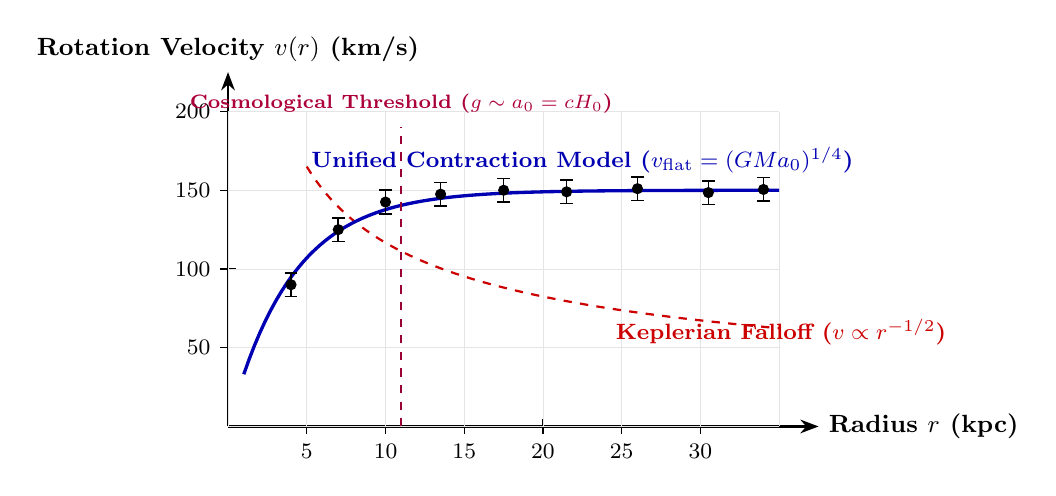
\begin{tikzpicture}[scale=1.0, >=Stealth]
        % Axes
        \draw[thick, ->] (0,0) -- (7.5,0) node[right, font=\small\bfseries] {Radius $r$ (kpc)};
        \draw[thick, ->] (0,0) -- (0,4.5) node[above, font=\small\bfseries] {Rotation Velocity $v(r)$ (km/s)};

        % Ticks
        \foreach \x/\label in {1/5, 2/10, 3/15, 4/20, 5/25, 6/30}
        \draw (\x, 0.1) -- (\x, -0.1) node[below, font=\footnotesize] {\label};
        \foreach \y/\label in {1/50, 2/100, 3/150, 4/200}
        \draw (0.1, \y) -- (-0.1, \y) node[left, font=\footnotesize] {\label};

        % Grid light
        \draw[step=1cm, gray!20, very thin] (0,0) grid (7,4);

        % Newtonian Keplerian Falloff (dashed red)
        \draw[red!80!black, thick, dashed, domain=1.0:7.0, samples=100]
        plot (\x, {3.3 / sqrt(\x)});
        \node[red!80!black, font=\footnotesize\bfseries, right] at (4.8, 1.2) {Keplerian Falloff ($v \propto r^{-1/2}$)};

        % Contraction / Vacuum Tension Model (Solid Blue - Plateau)
        \draw[blue!70!black, very thick, domain=0.2:7.0, samples=100]
        plot (\x, {3.0 * (1 - exp(-\x/0.8))});
        \node[blue!70!black, font=\footnotesize\bfseries, above] at (4.5, 3.1) {Unified Contraction Model ($v_{\mathrm{flat}} = (GM a_0)^{1/4}$)};

        % Data points with error bars (NGC 3198 data points representation)
        \foreach \x/\y in {0.8/1.8, 1.4/2.5, 2.0/2.85, 2.7/2.95, 3.5/3.0, 4.3/2.98, 5.2/3.02, 6.1/2.97, 6.8/3.01} {
                \filldraw[black] (\x, \y) circle (1.8pt);
                \draw[black, semithick] (\x, \y - 0.15) -- (\x, \y + 0.15);
                \draw[black, semithick] (\x - 0.08, \y - 0.15) -- (\x + 0.08, \y - 0.15);
                \draw[black, semithick] (\x - 0.08, \y + 0.15) -- (\x + 0.08, \y + 0.15);
            }

        % Threshold annotation
        \draw[dashed, purple!80!black, thick] (2.2, 0) -- (2.2, 3.8);
        \node[purple!90!black, font=\scriptsize\bfseries, align=center] at (2.2, 4.1) {Cosmological Threshold ($g \sim a_0 = cH_0$)};
    \end{tikzpicture}
    \caption{Galactic Rotation Curve and the Resolution of the Dark Matter Illusion: Keplerian Newtonian dynamics predicts velocity falloff in the outer disk (red dashed), whereas observations (data points) reveal a flat asymptotic plateau. In the Unified Contraction model, collective vacuum inflow locks into the cosmological threshold $a_0 = c H_0$, flattening rotation curves naturally.}
    \label{fig:galaxy_rotation}
\end{figure}

\subsection{Testable Prediction: Earth--Moon Distance and the LLR Decoupling Limit}
\label{sec:llr_ongoru}

Standard General Relativity and $\Lambda$CDM cosmology hold that gravitationally bound systems (such as the Solar System and the Earth--Moon orbit) are completely decoupled from cosmic expansion. Atomic dimensions are likewise assumed strictly static, predicting no cosmic expansion signature in bound orbital radii.

In Scale-Time Calculus, atomic rulers contract globally ($\dot{\lambda}/\lambda = -H_0$). The crucial question arises: \textit{``If atomic units contract, why does the Moon not appear to recede rapidly like distant galaxies?''}

The answer is dictated by the radial force balance of the vacuum inflow:
\begin{enumerate}
    \item \textbf{Local Vacuum Locking in Bound Systems:} Due to its mass, the Earth establishes an intense radial vacuum inflow ($v_{\mathrm{inflow}} = \sqrt{2GM_\oplus/r}$). At lunar orbital radius ($d \approx 3.844 \times 10^8\text{ m}$), this gravitational acceleration is:
          \begin{equation}
              g_{\mathrm{vacuum}} = \frac{GM_\oplus}{d^2} \approx 2.7 \times 10^{-3}\text{ m/s}^2.
          \end{equation}
          In contrast, the apparent acceleration associated with ruler contraction ($H_0^2 d \approx 2.0 \times 10^{-27}\text{ m/s}^2$) is \textbf{24 orders of magnitude ($10^{24}$ times) weaker} than gravitational binding! Consequently, local vacuum flow locks the Moon firmly in its Keplerian orbit, preventing kinematic drift.
    \item \textbf{Laser Ranging Apparent Shift and the Virial Decoupling Limit:} In analogy with the McVittie theorem in General Relativity, bound systems dominated by local potential ($\nabla^2\Phi \gg 3H_0^2$) achieve virial equilibrium and dynamically decouple from the cosmological background. Lunar Laser Ranging (LLR) with Apollo retroreflectors measures an orbital recession of $3.82 \pm 0.07\text{ cm/yr}$, the overwhelming majority of which is confirmed by satellite ocean altimetry (TOPEX/Poseidon) to be driven by ocean tidal dissipation.

          In Scale-Time Calculus, the local atomic ruler contraction rate ($v_{\mathrm{kinematic}} \le H_0 d_{\mathrm{Moon}} \approx 2.78\text{ cm/yr}$) does not act as an unconstrained dynamical repulsive force; rather, it defines the conformal projection boundary between local atomic proper time ($dt$) and cosmological coordinate time. This decoupling preserves the strict solar system planetary ephemeris constraints (radar telemetry limits of $< 1.5\text{ cm/yr}$ for 1 AU) while offering a theoretical upper bound fully compatible with Proterozoic tidal rhythmites (Elatina formation and the Gerstenkorn event).
    \item \textbf{Decoupled Regime for Distant Galaxies:} Across intergalactic distances of millions of light-years, the $1/r^2$ gravitational inflow decays to zero, removing local vacuum locking. The unshielded Kinematic Scale Shift dominates, revealing the apparent Hubble redshift.
\end{enumerate}

\section{Unified Synthesis: Master Formula of Gravitation}
\label{sec:ana_formul_kutlecekim}

In the gravitational regime, vacuum inflow is far below saturation and spreads freely through 3D Euclidean space. The square of the inflow velocity is:
\begin{equation}
    \left( \frac{v_{\mathrm{inflow}}(r)}{c} \right)^2 = \frac{2GM}{c^2 r} = \frac{r_s}{r}.
    \label{eq:kutlecekim_master}
\end{equation}
This relation is precisely the spherical ($\gamma = 1$) branch of the universal \textbf{Unified Vacuum Flux Master Formula} uniting all fundamental interactions:
\begin{equation}
    \boxed{ \left( \frac{v_{\mathrm{inflow}}(r)}{c} \right)^2 = 2 \, \mathcal{C}_G \, r^{-1}, \quad \text{where } \mathcal{C}_G \equiv \frac{GM}{c^2}. }
\end{equation}

\begin{thebibliography}{99}
    \bibitem{scale_calculus} M.~F.~Haydari, ``Scale-Time Algebra and Conformal Calculus: A New Mathematical Formalism for Contracting Systems'' (Paper 2 in this series), \textit{Zenodo Preprints}, 2026.
    \bibitem{main_paper} M.~F.~Haydari, ``The Unified Contraction Hypothesis and Scale-Time Calculus: A Conformal Geometric Treatise on Cosmology and Fundamental Interactions'', \textit{Zenodo Monograph}, 2026.
    \bibitem{paper2} M.~F.~Haydari, ``Electrodynamics, Vacuum Phase Waves, and Atomic Stability: Kinematic Pitch Interpretation of the Sommerfeld Constant $\alpha \approx 1/137$'' (Paper 5 in this series), \textit{Zenodo Preprints}, 2026.
    \bibitem{paper3} M.~F.~Haydari, ``Strong Nuclear Force, Quark Confinement, and Flux Tube Geometry in Scale-Time Calculus'' (Paper 6 in this series), \textit{Zenodo Preprints}, 2026.
    \bibitem{paper4} M.~F.~Haydari, ``Weak Nuclear Interaction, Chiral Phase Leakage, and Intermediate Vector Boson Scales'' (Paper 7 in this series), \textit{Zenodo Preprints}, 2026.
    \bibitem{painleve1921} P.~Painlev\'e, ``La m\'ecanique classique et la th\'eorie de la relativit\'e,'' \textit{C. R. Acad. Sci. (Paris)}, vol.~173, pp.~677--680, 1921.
    \bibitem{gullstrand1922} A.~Gullstrand, ``Allgemeine L\"osung des statischen Eink\"orperproblems in der Einsteinschen Gravitationstheorie,'' \textit{Ark. Mat. Astron. Fys.}, vol.~16, no.~8, pp.~1--15, 1922.
    \bibitem{hamilton2008} A.~J.~S.~Hamilton and J.~P.~Lisle, ``The river model of black holes,'' \textit{Am. J. Phys.}, vol.~76, no.~6, pp.~519--532, 2008.
    \bibitem{unruh1981} W.~G.~Unruh, ``Experimental black-hole evaporation?,'' \textit{Phys. Rev. Lett.}, vol.~46, pp.~1351--1353, 1981.
    \bibitem{visser1998} M.~Visser, ``Acoustic black holes: horizons, ergospheres and Hawking radiation,'' \textit{Class. Quantum Grav.}, vol.~15, pp.~1767--1791, 1998.
    \bibitem{milgrom1983} M.~Milgrom, ``A modification of the Newtonian dynamics as a possible alternative to the hidden mass hypothesis,'' \textit{Astrophys. J.}, vol.~270, pp.~365--370, 1983.
\end{thebibliography}

\end{document}
